\newpage
\chapter{Les réplicons extra-chromosomiques essentiels}\label{chap1b}
\lhead{\emph{Les réplicons extra-chromosomiques essentiels}}

\section{Découverte et premières caractérisations de génomes multipartites bactériens}
     
      Le modèle du génome bactérien que nous avons introduit dans le chapitre précédent repose essentiellement sur l'architecture du génome d'\textit{E. coli}, formé d'un unique chromosome circulaire et, éventuellement, de plasmides. Cette organisation proposée dans les années 1950 \citep{wollman1956conjugation} et mise en évidence par autoradiographie  du génome de \textit{E. coli} \citep{cairns1963chromosome}, fut plus tard retrouvée lors de l'étude de génomes additionnels, \textit{i.e.}, \textit{Bacillus subtilis}, et s'imposa alors comme la règle chez les bactéries. Ce modèle n'est cependant pas valide pour toutes les bactéries. Les génomes bactériens peuvent comporter plusieurs réplicons de type chromosomique (\textbf{génome multipartite}), et les réplicons bactériens, chromosomes et plasmides, pouvent être circulaires ou linéaires \citep{baril1989linear,kolsto1997dynamic,casjens1998diverse}.\\
       Les premières preuves de génomes multipartites bactériens apparurent avec la caractérisation par électrophorèse en champ pulsé du génome de \textit{Rhodobacter sphaeroides} à la fin des années 1980, qui permit de réaliser la seconde carte physique de génome  bactérien, après celle d'\textit{E. coli} \citep{suwanto1989physical,suwanto1989physicala}. Ces résultats mirent en évidence que deux des réplicons de \textit{R. sphaeroides} portent des gènes codant des ARNr et sont strictement essentiels pour la bactérie. Ces réplicons furent alors désignés par les termes de chromosome primaire (pour le plus grand) et chromosome secondaire \citep{suwanto1989physical}. Ces approches méthodologiques ont par la suite mis en évidence la présence de multiples réplicons essentiels chez \textit{Leptospira interrogans} \citep{zuerner1993comparison}, \textit{Brucella} \citep{michaux1993presence}, \textit{Pseudoalteromonas haloplanktis} \citep{lanoil1996marine}, \textit{Burkholderia} \citep{rodley1995physical} et \textit{Vibrio cholerae} \citep{trucksis1998vibrio}.\\           
        Depuis, les progrès des techniques de séquençage ont permis d'obtenir les séquences complètes de milliers de génomes bactériens révélant ainsi une grande diversité quant au nombre de chromosomes et de plasmides par complément génomique, à leurs tailles, et à leurs topologies, ainsi qu'une hétérogénéité de répartition de ces caractéristiques parmi les différentes lignées bactériennes \citep{casjens1998diverse,Mackenzie2004}. L'étude du catalogue, toujours plus important, des génomes dont la séquence complète est disponible, ainsi que la compréhension du développement bactérien \textit{in vivo} et \textit{in vitro} montrent qu'il existe non seulement des réplicons accessoires de taille et de complexité génomiques proches de celles des chromosomes mais que la limite entre réplicon essentiel et réplicon accessoire peut être difficile à définir \citep{Mackenzie2004}.\\ 
	Pour certains auteurs, le statut des réplicons dépend avant tout des caractéristiques structurales de ceux-ci  \citep{harrison2011bacterial}. Des études des structures d'\textit{ori} de chromosomes secondaires ont montré de grandes similarités avec les \textit{ori} de mégaplasmides, rapprochant ces deux types de réplicons d'un point de vue évolutif et fonctionnel. Différents modules génétiques ou gènes spécifiques, typiques des plasmides (tels que les gènes impliqués dans la conjugaison), sont retrouvés sur les chromosomes secondaires. Une autre ambiguïté provient de la distinction classique, conforme au dogme du chromosome bactérien unique, entre les différents réplicons essentiels d'un génome bactérien multipartite: on parle alors d'un chromosome \textit{primaire} et de chromosome secondaire ou mégaplasmide \citep{MacLellan2004} pour les \textbf{R}éplicons \textbf{E}xtra-\textbf{C}hromosomiques \textbf{E}ssentiels (\textbf{RECE}) sur la base de caractéristiques telles que la taille des réplicons, le nombre de gènes ou la présence de gènes essentiels.


\section{Diversité actuelle des génomes multipartites bactériens}\label{diversite}
	\definecolor{deepblue}{rgb}{1,0.5,0}
	Les occurrences de génomes multipartites dans les différentes lignées bactériennes sont hautement variables. Les génomes multipartites sont disséminés de façon irrégulière à travers la phylogénie des bactéries (Figure \ref{figphylgeco}). Les Protéobactéries semblent être leur phylum de prédilection car on les observe beaucoup plus fréquemment chez les Alpha-, Bêta- et Gamma-protéobactéries. Chez les Alpha-protéobactéries, jusqu'à 10 genres bactériens différents comportent au moins une espèce à génome multipartite. Par contre, le phylum des Firmicutes n'en comporte que peu  (deux génomes multipartites répertoriés) au regard du nombre d'espèces dont le génome a été complètement séquencé (745 espèces dans 90 genres taxonomiques). Néanmoins, la présence de réplicons secondaires essentiels a été relevée dans la plupart des lignées bactériennes majeures telles que les Spirochètes (\textit{Leptospira}), les Bacteroidetes (\textit{Prevotella}), les Firmicutes (\textit{Butyrivibrio} et \textit{Clostridium}), ou encore les Cyanobactéries (\textit{Anabaena} et \textit{Cyanothece}) (Table \ref{tabess}; Annexe \ref{AppendiceA}). Chez les Protéobactéries, 19 genres sur 231 contiennent au moins une espèce possédant un génome multipartite, pour seulement deux des 90 genres de firmicutes, soit quatre fois moins. Cela traduit peut-être simplement un échantillonnage déséquilibré vers les organismes pathogènes ou symbiotiques pour des raisons médicales et/ou économiques. L'écologie et le génome d'espèces telles que \textit{Candidatus} Chloroacidobacterium thermophilum \citep{GarciaCostas2012} ou \textit{Ilyobacter polytropus} \citep{Sikorski2010} en sont des contre-exemples, témoignant de l'effort récent pour étendre l'acquisition de données de séquences aux bactéries de l'environnement et à l'ensemble des bactéries, et plus généralement du vivant.  \\

\begin{figure}[H]
	\begin{center}
	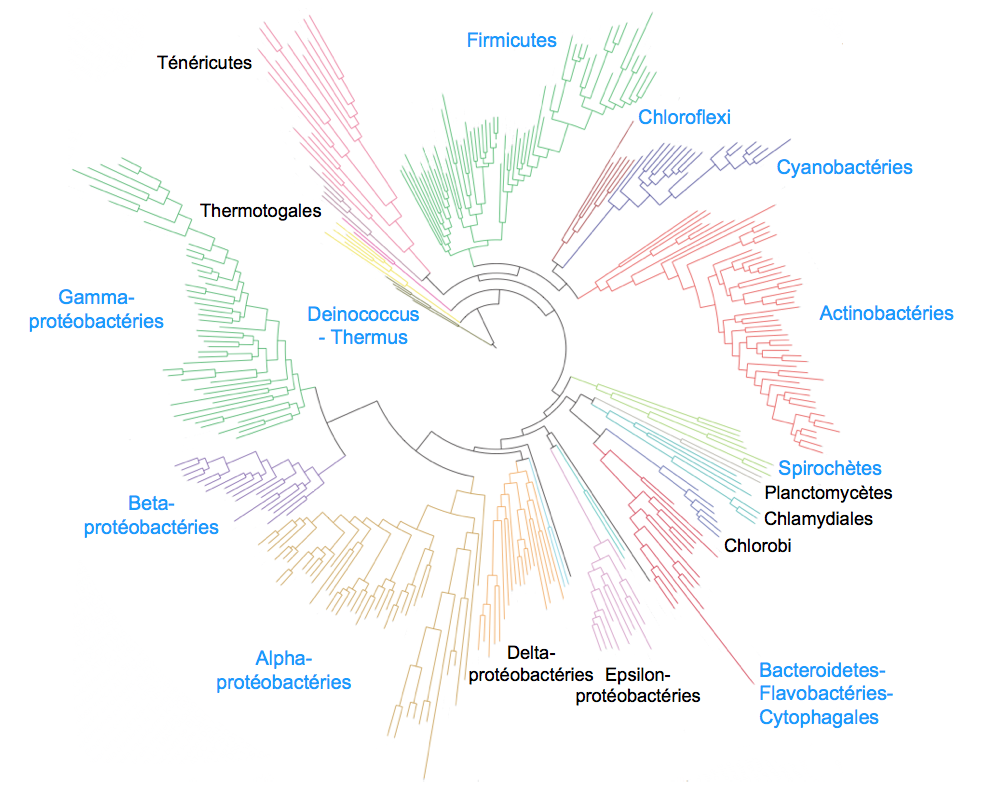
\includegraphics[height=0.4\textheight]{./img/figphylgeco.png}
	\caption[Distribution des génomes multipartites dans le domaine Bacteria]{Distribution des génomes multipartites (bleu) dans le domaine Bacteria.}\label{figphylgeco}
	 \end{center}
 \end{figure} 

	L'existence de RECE n'est pas corrélée avec la présence ou l'absence de plasmide au sein d'un génome. Ils peuvent être:
\begin{description}
      \item[$\bullet$] observés ponctuellement au sein d'une lignée (cas des Alteromonadales où seules deux espèces de \textit{Pseudoalteromonas} possèdent un génome multipartite,
      \item[$\bullet$] retrouvés chez un grand nombre d'espèces d'une même lignée sans être ubiquiste (cas des Rhizobiales où de nombreuses espèces (\textit{Brucella}, \textit{Ochrobactrum}, \textit{Rhizobium} et \textit{Sinorhizobium}), mais pas toutes (\textit{Bradyrhizobium}, \textit{Mesorhizobium}...) ont des génomes multipartites,
      \item[$\bullet$] ou encore présents dans toutes les espèces d'une lignée (cas des Vibrionales).
\end{description}
       La taille des RECE varie considérablement, le plus petit (0,27 Mb) étant trouvé chez \textit{Leptospira biflexa} et le plus grand  (3,7 Mb) chez \textit{Burkholderia gladioli}. Enfin, même si la majorité des RECE a une topologie circulaire, certains, dans les génomes de \textit{Agrobacterium} et de \textit{Cyanothece}, sont linéaires.\\
      Les espèces à génomes multipartites possèdent des écologies variées, pouvant être pathogènes (\textit{Brucella}, \textit{Vibrio}, \textit{Burkholderia}), des symbiotes de plantes (\textit{Burkholderia}, \textit{Rhizobium}) ou d'animaux (\textit{Vibrio}, \textit{Photobacterium}), avoir une écologie marine (\textit{Pseudoalteromonas}, \textit{Vibrio}, \textit{Anabaena}) ou être extrêmophiles (\textit{Deinococcus}), par exemple. 
     

\section{Essentialité}\label{chrIIess}
	L'essentialité d'un réplicon dépend directement de celle des gènes qu'il code. Ainsi, selon la définition d'Ochman \citep{Ochman2002}, un réplicon est considéré comme un chromosome s'il porte au moins un gène considéré comme essentiel à la vie de la bactérie, présent en copie unique dans le génome. La notion de gène essentiel pour un organisme relève du concept de ``génome minimal" où 100 à 300 gènes sont absolument indispensables à la survie et au développement de l'organisme bactérien \citep{Koonin2000,Glass2006}. Ces gènes codent majoritairement des protéines impliquées dans la réplication de l'ADN, la transcription des gènes, la traduction, et l'utilisation du carbone et de l'énergie \citep{MacLellan2004}. Le statut de chromosome s'applique ainsi au second réplicon de \textit{Rhodobacter sphaeroides} car il porte des gènes d'ARNr et de certaines enzymes du métabolisme primaire \citep{suwanto1989physical}. Le statut de chromosome a également été accordé aux réplicons de \textit{Butyrivibrio proteoclasticus} \citep{Kelly2010}, \textit{Nocardiopsis dassonvillei} \citep{Sun2010} et \textit{Ilyobacter polytropus} \citep{Sikorski2010}, car ils portent des gènes codant des ARNr et des ARN de transfert (\textbf{ARNt}). Le chromosome secondaire de \textit{Rhizobium radiobacter} (anciennement \textit{Agrobacterium tumefaciens}) possède la plupart des gènes codant des régulateurs transcriptionnels et des transporteurs ABC en plus de gènes d'ARNt et ARNr \citep{MacLellan2004}. De même, le second réplicon essentiel de \textit{Sinorhizobium meliloti} porte une part significative des gènes impliqués dans le métabolisme cellulaire et l'exploitation des sources de carbone et d'azote présentes au niveau du sol \citep{MacLellan2004}.\\
      La distinction entre chromosome et plasmide n'est cependant pas aussi tranchée et ne peut reposer sur la seule présence (chromosome) ou absence (plasmide) de gènes``marqueurs" sans copie sur un autre réplicon du genome. Certains réplicons plasmidiques portent des gènes essentiels \citep{Yeoman2011}, les plus fréquemment observés étant des opérons ARNr \citep{baril1992scattering,salanoubat2002genome,moran2004genome,pohlmann2006genome}. À l'inverse, il existe des RECE qui n'en codent pas \citep{Heidelberg2000,Nascimento2004}. Par ailleurs, de nombreux réplicons bien que plasmidiques contribuent significativement à la \textit{\textbf{fitness}} de leur hôte \citep{MacLellan2004,Krone2007,lopez2012rhizobial}, le terme \textit{fitness} désignant ici ce qui a rapport avec les capacités de survie et de développement d'un organisme bactérien à court, moyen et long terme, dans son (ou ses) habitat(s) naturel(s). Du fait de la difficile tâche de mesurer la contribution d'un gène ou d'un réplicon à la \textit{fitness} d'un organisme \citep{Mackenzie2004}, \textbf{il devient délicat de différencier chromosomes et plasmides uniquement sur la contribution d'un réplicon à la \textit{fitness} de l'organisme bactérien.} \\
      En règle générale, la distribution en gènes essentiels est largement déséquilibrée en faveur d'un réplicon principal (\textbf{chromosome primaire} ou \textbf{chr}) \citep{Mackenzie2004}, même si certains RECE font exception \citep{Choudhary2004,Egan2005,Choudhary2007}. Parmi les RECE recensés, on observe différents cas de figure (Tableau \ref{tabess}), empêchant l'inférence directe de règles quant à la distribution de gènes essentiels en nombre et type sur les RECE.   

\newpage

%%%%%%%%%%%%%%%%%%%%%%%%%%%%%%%%%%%%%%%%%%%%%%%%%%%%%%%%%%%%%%%%%%%%%%%%%
 \begin{longtable}{@{\hspace{-2cm}} >{\footnotesize\itshape}p{0.1\textwidth} | >{\small\flushleft}p{0.045\textwidth} | >{\small}p{0.04\textwidth} |>{\small}p{0.04\textwidth} | >{\footnotesize}p{0.6\textwidth} | >{\scriptsize}p{0.2\textwidth} @{\hspace{0.5cm}}}
    \endhead
	\caption[Caractéristiques essentielles des RECE]{Caractéristiques essentielles des RECE selon le genre de leur hôte.\\Source: génomes complets disponibles dans RefSeq au 23/11/2013. M: nombre de génomes multipartites rapporté au nombre total de génomes séquencés pour un genre bactérien donné. ARNr/ARNt: présence de gènes ARNr/ARNt. Référence: la première référence correspond à la première caractérisation du génome multipartite du genre quand elle est disponible, sinon les numéros d'accession des BioProjects (NCBI) sont fournis.}\label{tabess}\\
	  \multicolumn{1}{@{\hspace{-2cm}}l} {\small\textbf{Lignée}} & \multicolumn{1}{ l} {\small\textbf{M}}&\multicolumn{1}{ p{0.04\textwidth}} {\small\textbf{ARNt}}&\multicolumn{1}{ @{\hspace{0.3cm}}p{0.04\textwidth}@{\hspace{-0.3cm}}} {\small\textbf{ARNr}} & \multicolumn{1}{ c} {\small\textbf{Autres caractéristiques}} & \multicolumn{1}{ l} {\small\textbf{Références}}\\
	\endfirsthead
	\multicolumn{1}{@{\hspace{-2cm}}l}{\small\textbf{Lignée}} & \multicolumn{1}{ l} {\small\textbf{M}}&\multicolumn{1}{ p{0.04\textwidth}} {\small\textbf{ARNt}}&\multicolumn{1}{ @{\hspace{0.3cm}}p{0.04\textwidth}@{\hspace{-0.3cm}}} {\small\textbf{ARNr}} & \multicolumn{1}{ c} {\small\textbf{Autres caractéristiques}} & \multicolumn{1}{ l} {\small\textbf{Références}}\\
	\endhead
	\hline
	\multicolumn{1}{@{\hspace{-2cm}}} {} \\
	\multicolumn{1}{@{\hspace{-2cm}} p{0.15\textwidth}} {\textbf{Alphaprotéobactéries}}\\
	Agrobacterium & 4/4 & Oui & Oui & Présence de \textit{minCDE}, de gènes liés à la réplication de l'ADN, au métabolisme, à l'infection et de régulateurs transcriptionnels & \citep{wood2001genome,goodner2001genome,allardet1993presence},\citep{MacLellan2004,Slater2009} \\
	\hline
	Asticcacaulis & 1/1 & Oui & Oui & \centering - & PRJNA55641 \\
	\hline
	Brucella & 18/18 & Oui & Oui & Présence de l'opéron \textit{minCDE} et différents gènes d'ARNt-synthétases & \citep{Jumas-Bilak1998,paulsen2002brucella,delvecchio2002genome},\citep{MacLellan2004} \\
	\hline
	Ochrobactrum & 1/1 & Oui & Oui & Présence d'homologues de \textit{minC} et \textit{minD} & \citep{Slater2009,chain2011genome} \\
	\hline
	Paracoccus & 1/1 & Oui & Non & Présence de nombreux gènes d'ARNt-synthétases ou méthyltransférases & PRJNA58187 \\
	\hline
	Rhodobacter & 4/5 & Oui & Oui & Présence de nombreux gènes typiquement chromosomiques liés au métabolisme; Sous-représentation des gènes liés à la division cellulaire  & \citep{kiley1988molecular,suwanto1989physical,mackenzie2001home},\citep{Choudhary2004,Mackenzie2004,Mackenzie2007,Choudhary2007} \\
	 \hline
	Sinorhizobium & 1/1 & Non & Non & Présence de \textit{minCDE}, de gènes liés à l'infection et au métabolisme, et de régulateurs transcriptionnels; RECE similaire aux mégaplasmides des Rhizobiaceae  & \citep{kaneko2000complete},\citep{MacLellan2004,Slater2009} \\
	\hline
	Sphingobium & 2/2& Oui & Oui & Présence de gènes codant diverses enzymes essentielles, des sous-unités d'une ARN polymérase et des gènes impliqués dans le métabolisme et l'adaptation à l'environnement & \citep{nagata2010complete,Copley2012} \\
	\hline
	\multicolumn{1}{@{\hspace{-2cm}}} {}\\
	\multicolumn{1}{@{\hspace{-2cm}} p{0.15\textwidth}} {\textbf{Bêtaprotéobactéries}}\\
	Burkholderia & 39/40 & Oui & Oui & Présence de nombreux gènes impliqués dans le métabolisme primaire et la synthèse d'acides aminés; Répartition des gènes essentiels variable selon les espèces. Pour l\textit{B. cenocepacia}, ratio (chromosome/RECE-1/RECE-2) en gènes essentiels de l'ordre de 250/50/50 & \citep{Songsivilai2000,komatsu2003distribution,nierman2004structural},\citep{Guo2010} \\
	\hline
	Cupriavidus/ Ralstonia & 6/13 & Oui & Oui & Présence d'un gène d'une sous-unité de la polymérase et d'un facteur d'élongation avec des paralogues sur le chromosome. Présence de nombreux gènes impliqués dans l'infection des plantes et la formation du flagelle. & \citep{salanoubat2002genome},\citep{MacLellan2004,pohlmann2006genome,amadou2008genome} \\
	\hline
	Variovorax & 2/3 & Non & Oui & chromosome largement favorisé en gènes essentiels  & \citep{han2011complete} \\
	\hline
	\multicolumn{1}{@{\hspace{-2cm}}} {}\\
	\multicolumn{1}{@{\hspace{-2cm}} p{0.15\textwidth}} {\textbf{Gammaprotéobactéries}} \\
	Pseudo-alteromonas  & 2/3 & Non & Non & présence de gènes essentiels \textit{hisE} et \textit{gcpE}, ainsi que des gènes du métabolisme de l'histidine sur le RECE de \textit{P. haloplanktis}; génomes multipartites des deux espèces très similaires & \citep{medigue2005coping},\citep{Qin2011} \\
	\hline
	Vibrio  & 28/28 & Oui & Oui & Nombreux gènes impliqués dans la réparation de l'ADN, gènes impliqués dans le métabolisme énergétique, gènes de protéines ribosomales, d-sérine désaminase et thréonyl-tRNA synthétase; quasi majorité des gènes d'ARNr portée par le chromosome & \citep{trucksis1998vibrio,yamaichi1999physical},\citep{tagomori2002comparison,MacLellan2004,Heidelberg2000} \\
	\hline
	Aliivibrio  & 1/1& Oui & Oui & Génome proche du celui des \textit{Vibrio} & \citep{hjerde2008genome} \\
	\hline
	Photobacterium  & 1/1 & Oui & Oui & RECE en moyenne 25\% plus grand que ceux de \textit{Vibrio} & \citep{vezzi2005life} \\
     \hline
	\multicolumn{1}{@{\hspace{-2cm}}} {}\\
     \multicolumn{1}{@{\hspace{-2cm}} p{0.15\textwidth}} {\textbf{Acidobactéries}}\\
     Candidatus \textnormal{\mbox{Chloroacido-} \mbox{bacterium} \mbox{thermophilum}} & 1/1 & Non & Oui & Présence de gènes essentiels impliqués dans la chlorophototrophie & \citep{GarciaCostas2012}\\
	\hline
	\multicolumn{1}{@{\hspace{-2cm}}} {}\\
      \multicolumn{1}{@{\hspace{-2cm}} p{0.15\textwidth}} {\textbf{Actinobactéries}} \\
      Nocardiopsis & 1/1 & Oui & Oui & \centering - & \citep{Sun2010} \\
      \hline
	\multicolumn{1}{@{\hspace{-2cm}}} {}\\
      \multicolumn{1}{@{\hspace{-2cm}} p{0.15\textwidth}} {\textbf{Bacteroidetes}} \\
      Prevotella & 3/6 & Oui & Oui & \centering - & PRJNA47507, PRJNA51377, PRJNA65091, PRJNA163151\\
      \hline
	\multicolumn{1}{@{\hspace{-2cm}}} {}\\
      \multicolumn{1}{@{\hspace{-2cm}} p{0.15\textwidth}} {\textbf{Chloroflexi}}\\
      Sphaerobacter & 1/1 & Oui & Oui & \centering - &\citep{pati2010complete} \\
	\hline
	\multicolumn{1}{@{\hspace{-2cm}}} {}\\ 
	\multicolumn{1}{@{\hspace{-2cm}} p{0.15\textwidth}} {\textbf{Cyanobactéries}}\\
	Anabaena & 1/3 & Non & Oui & Présence de génes d'ARNt synthétases et ARNr méthyltransférases & \citep{Wang2012a} \\
	\hline
	Cyanothece & 1/6 & Non & Non& Présence de génes d'ARNt synthétases; Nombreux gènes singuliers du RECE linéaire & \citep{Welsh2008} \\
     \hline
     Thermobaculum & 1/1 & Non & Non & \centering - & \citep{Kiss2010} \\
     \hline
	\multicolumn{1}{@{\hspace{-2cm}}} {}\\
     \multicolumn{4}{@{\hspace{-2cm}} p{0.3\textwidth}} {\textbf{Deinococcus-Thermus}}\\
     Deinococcus & 1/7 & Oui & Oui & Présence de gènes d'ARNt synthétases; Nombreux gènes spécialisés dans l'adaptation à l'environnement & \citep{White1999}, \citep{MacLellan2004} \\
     \hline
	\multicolumn{1}{@{\hspace{-2cm}}} {}\\
     \multicolumn{1}{@{\hspace{-2cm}} p{0.15\textwidth}} {\textbf{Firmicutes}}\\
     Butyrivibiro & 1/2 & Oui & Oui & Présence des gènes essentiels \textit{acpD} et \textit{msrA}; gènes essentiels présents sur un plasmide de \textit{B. proteoclasticus} & \citep{Kelly2010},\citep{Yeoman2011} \\
     \hline
     Clostridium & 1/62 & Oui & Non & \centering - & DS,\citep{he2010evolutionary} \\
     \hline
	\multicolumn{1}{@{\hspace{-2cm}}} {}\\
      \multicolumn{1}{@{\hspace{-2cm}} p{0.15\textwidth}} {\textbf{Fusobactéries}}\\
      Ilyobacter & 1/1 & Oui & Oui & \centering - &\citep{Sikorski2010}\\
	\hline
	\multicolumn{1}{@{\hspace{-2cm}}} {}\\
	\multicolumn{1}{@{\hspace{-2cm}} p{0.15\textwidth}}{\textbf{Spirochètes}} \\
	Leptospira & 7/7 & Non & Non & Présence de \textit{ndh} (NADH déshydrogénase), \textit{gltB} (glutamate synthétase) et \textit{asd} (aspartate semialdéhyde dehydro-génase) & \citep{zuerner1993comparison,ren2003unique},\citep{nascimento2004comparative,bulach2006genome,Picardeau2008}\\
\end{longtable}
%%%%%%%%%%%%%%%%%%%%%%%%%%%%%%%%%%%%%%%%%%%%%%%%%%%%%%%%%%%%%%%%%%%%%%%%%

	Outre les RECE annotés, le statut de certains réplicons est ambigu. Bien que classés parmi les (méga)plasmides sur la base de caractéristiques structurales ou fonctionnelles, ils semblent jouer un rôle de RECE ou paraissent en posséder certaines caractéristiques. Ainsi, chez les Alphaprotéobactéries, différents plasmides de \textit{Rhizobium elti} (Rhizobiales) présentent de nombreuses caractéristiques (stabilité, essentialité...) de RECE \citep{Landeta2011}, ainsi que chez \textit{Azospirillum} (Rhodospirillales), bactéries promouvant la croissance de diverses plantes \citep{wisniewski2011azospirillum,Acosta-Cruz2012}. Différents plasmides des \textit{Roseobacter} seraient également des RECE sur la base de caractéristiques structurales (\textit{ori}, pourcentage en G+C) des réplicons \citep{Petersen2013}. 

\section{Régulation et intégration des RECE dans le cycle cellulaire}\label{model}
	La présence d'un chromosome additionnel dans un génome ajoute des contraintes à l'organisme et requiert des mécanismes moléculaires supplémentaires permettant son intégration dans le cycle cellulaire \citep{Venkova-Canova}. Par opposition à un plasmide, un RECE doit être répliqué une unique fois en un moment précis du cycle cellulaire et doit être activement ségrégé lors de la division cellulaire  \citep{Egan2005}.\\ 
	
Le modèle le plus populaire d'intégration d'un RECE dans le génome est l'adaptation des systèmes de réplication et ségrégation d'un mégaplasmide au cycle cellulaire \citep{Heidelberg2000,MacLellan2004}. Les mécanismes les mieux décrits sont ceux de \textit{V. cholerae} où l'hypothèse plasmidique d'origine du RECE est postulée \citep{egan2003distinct}. Il a été montré que le chromosome et le RECE de \textit{V. cholerae} se répliquent une fois par cycle cellulaire \citep{srivastava2007selective,stokke2011replication}. La réplication débute après celle du chromosome et termine en synchronisation avec lui \citep{rasmussen2007two,stokke2011replication}, et implique des régulateurs communs \citep{Egan2005,demarre2010dna}. Le RECE de \textit{V. cholerae} possède deux gènes spécifiques, \textit{rtcB} codant RtcB, protéine initiatrice de la réplication du RECE des \textit{Vibrionaceae} et \textit{Photobacteriaceae} à l'instar de DnaA pour la réplication du chromosome, et \textit{rtcA} intervenant dans la régulation de RctB \citep{duigou2006independent}. RtcB est de plus régulée par le chromosome par fixation à des motifs spécifiques localisés sur ce dernier \citep{baek2014chromosome}, ce qui démontre l'implication du chromosome dans la réplication du RECE et, partant, l'intégration du RECE dans le cycle cellulaire et le génome stable de \textit{V. cholerae}. La réplication du RECE est inhibée par une séquence adjacente à l'\textit{ori}, \textit{inc}, et semble aussi sous le contrôle de DnaA et Dam de par la présence de boîtes DnaA et de motifs GATC à l'origine \citep{egan2006autorepression,saint2008excess}. Interviennent également des mécanismes de \textit{handcuffing}, typiques des plasmides \citep{egan2003distinct,Egan2005,zakrzewska2007regulation}. Le RECE possède son propre système de partition ParA2/ParB2, essentiel à la maintenance du RECE, qui interagit (\textit{via} ParB2) avec \textit{rtcA} et RtcB, liant ainsi  réplication et ségrégation du RECE \citep{yamaichi2011regulatory}. Les mécanismes moléculaires de résolution de dimère de RECE font intervenir les mêmes résolvases XerC et XerD que pour le chromosome en le liant au cycle cellulaire par l'intermédiaire de l'action de FtsK \citep{Val2008}. FtsK est, pour le RECE comme pour le chromosome de \textit{V. cholerae} guidé par des motifs KOPS \citep{Val2008}.  \\

	 Le modèle de réplication/ségrégation de \textit{V. cholerae} met en évidence des adaptations génomiques spécifiques du RECE: présence de régulateurs et protéines supplémentaires spécifiques, motifs structuraux de régulation, qui semblent être le fruit de la modification d'un mégaplasmide chez l'ancêtre commun des \textit{Vibrio}\citep{Heidelberg2000}. Cependant, ce modèle est actuellement le seul décrivant en quelques détails les spécificités génomiques permettant l'intégration des RECE dans le cycle cellulaire, et ne peut \textit{de facto} être directement généralisé à tous les RECE.\\
	Les autres mécanismes d'intégration d'un réplicon additionnel dans le cycle cellulaire concernent principalement les spécificités de la partition chez les génomes multipartites des Burkholderiales, avec des adaptations des systèmes parABS des RECE en comparaison de ceux des chromosomes et des plasmides \citep{Dubarry2006a,Livny2007,Passot2012}. En particulier, ces adaptations impliquent une séquence \textit{parS} spécifique des RECE et une régulation des systèmes de partition des RECE de \textit{B. cenocepacia} par opposition à un système de partition plasmidique classique \citep{Dubarry2006a}.


\section{Origine évolutive}\label{chrIIori}
	Quelles sont donc les structures génétiques ancestrales expliquant la diversité actuelle des réplicons secondaires essentiels? D'un point de vue théorique, plusieurs hypothèses peuvent être envisagées:
	
\subsection*{Deux hypothèses sont principalement favorisées:}
\begin{description}
	 \item[H1] La scission chromosomique. Un unique réplicon se divise en plusieurs réplicons essentiels, faisant potentiellement intervenir des recombinaisons site-spécifiques (\textit{cf.} \S \ref{recom}). La coupure expérimentale d'un chromosome en deux molécules qui sont ensuite  transmises à la descendance a été décrite  \citep{guo2003natural,itaya1997experimental}. 
	 \item[H2]  L'adaptation d'un réplicon accessoire avec enrichissement progressif en gènes essentiels chromosomiques  \citep{Moreno1998,Mackenzie2004}. Cette hypothèse implique l'action de divers processus de recombinaisons génétiques entre chromosomes et plasmides, dont certains ont été identifiés et caractérisés \citep{Slater2009,Guo2010,maida2014origin}. Cette hypothèse est actuellement la plus généralement retenue pour rendre compte de l'existence de la plupart des génomes multipartites, en particulier de ceux des Protéobactéries \citep{Bavishi2010}. 
\end{description}
\subsection*{D'autres mécanismes ont été proposés:}
	 \begin{description}
	 \item[h1] Capture d'un chromosome externe \citep{Moreno1998,Mackenzie2004}. Il est alors nécessaire d'imaginer la formation d'une forme intermédiaire hybride, contenant plus d'un complément génomique.
	 \item[h2] Une réplication chromosomique inégale et/ou imparfaite faisant apparaître deux réplicons différents \citep{Moreno1998}, ce qui devrait se refléter dans la présence des régions dupliquées relativement abondantes dans le génome.
	 \item[h3]  Des mutations indépendantes sur des chromosomes d'espèces polyploïdes \citep{Moreno1998}, menant à une différentiation des chromosomes .
\end{description}

Même si les hypothèses h1, h2 et h3 sont vraisemblables, il n'existe pas à notre connaissance d'indice génomique indiscutable en leur faveur. Les hypothèses les plus susceptibles d'expliquer la formation des génomes multipartites les plus étudiés, avec les éléments les soutenant, sont synthétisés Table \ref{taborigin}.

%%%%%%%%%%%%%%%%%%%%%%%%%%%%%%%%%%%%%%%%%%%%%%%%%%%%%%%%%%%%%%%%%%%%%%%%%


\begin{longtable}{@{\hspace{-2cm}} >{\footnotesize\itshape}p{0.15\textwidth} | >{\bfseries\scriptsize}p{0.05\textwidth} | >{\scriptsize}p{0.50\textwidth} | >{\scriptsize}p{0.45\textwidth} @{\hspace{0.5cm}}}
	\caption[Origine évolutive des RECE d'après la littérature]{Origine évolutive des RECE d'après la littérature. \\ H: hypothèse(s) évolutive(s) des RECE.}\label{taborigin}\\
	\multicolumn{1}{@{\hspace{-2cm}} l} {\small\textbf{Lignée}} & \multicolumn{1}{p{0.03\textwidth}} {\small\textbf{Hyp}} & \multicolumn{1}{ @{\hspace{0.2cm}} l @{\hspace{-0.2cm}}} {\small\textbf{Origine de réplication}} & \multicolumn{1}{l} {\small\textbf{Autres caractéristiques}}\\
    \endfirsthead
		\multicolumn{1}{@{\hspace{-2cm}} l} {\small\textbf{Lignée}} & \multicolumn{1}{p{0.03\textwidth}} {\small\textbf{Hyp}} & \multicolumn{1}{ @{\hspace{0.2cm}} l @{\hspace{-0.2cm}}} {\small\textbf{Origine de réplication}} & \multicolumn{1}{l} {\small\textbf{Autres caractéristiques}}\\
     \endhead
     \hline
	\multicolumn{1}{@{\hspace{-2cm}}} {} \\
	\multicolumn{4}{@{\hspace{-2cm}} p{\textwidth}} {\textbf{Alphaprotéobactéries}}\\
	Asticcacaulis & ? & \multicolumn{2}{l}{\scriptsize Pas d'étude publiée de la structure génomique d'\textit{Asticcacaulis}}\\
	\hline
      Agrobacterium & H2 & Origine de réplication de type \textit{repABC} \citep{Slater2009} & Signatures génomiques proches de celles des plasmides;  ParA de type plasmidique \citep{MacLellan2004,Slater2009}.\\
     \hline
     
	Brucella & H2/ (H1/ h2/ h3) & Pour certains auteurs, l'\textit{ori} du RECE de \textit{B. melilentis} est similaire à celle du chromosome  \citep{delvecchio2002genome}, ce qui serait compatible avec les hypothèses H1,h2 et h3. Un locus \textit{repABC} est aussi présent \citep{MacLellan2004}; l'\textit{ori} du RECE  semble donc être homologue à celles de différents mégaplasmides et RECE de Rhizobiaceae \citep{paulsen2002brucella}. & Les ParA des RECE sont des homologues de protéines plasmidiques \citep{MacLellan2004} et de nombreux indices témoignent aussi d'un passé plasmidique proche de celui des autres mégaplasmides de la famille \citep{Slater2009}.\\
     \hline
      Ochrobactrum & H2 & Origine de réplication de type \textit{repABC} \citep{chain2011genome}. & Les génomes d'\textit{Ochrobactrum} et de \textit{Brucella} sont très proches phylogéniquement et génétiquement.\\
     \hline
	Paracoccus & ? & \centering - & Fréquents transferts entre les chromosomes et plasmides dans le genre \textit{Paracoccus} \citep{maj2013plasmids}. Certains plasmides des Rhodobacterales (dont fait partie \textit{Paracoccus}) possèdent des plasmides \textit{DnaA-like} caractéristiques \citep{petersen2011origin}\\
	\hline
	Rhodobacter & H1/ H2/ h2 & Présence d'un opéron \textit{repABC} \citep{Mackenzie2007} & Large duplication ancestrale entre le chromosome et le RECE \citep{Choudhary2004}. Expression génique faible  \citep{Mackenzie2007}. \\ 
	\hline
      Sinorhizobium & H2 & Origine de réplication de type \textit{repABC} \citep{barnett2001nucleotide,Slater2009} & RECE très proches des mégaplasmides des autres Rhizobiaceae \citep{Slater2009} \\
	\hline
      Sphingobium & H2 & Origine de réplication à proximité des gènes \textit{parA} et \textit{parB} ainsi que de \textit{repA} \citep{Copley2012} & Biais de distribution important des gènes essentiels en faveur du chromosome \citep{Copley2012}. \\ 
	\hline
	\multicolumn{1}{@{\hspace{-2cm}}} {} \\
	\multicolumn{4}{@{\hspace{-2cm}} p{\textwidth}} {\textbf{Bêtaprotéobactéries}}\\
	Burkholderia & H2 & Origine de réplication possédant des caractéristiques plasmidiques: proximité de \textit{parA} et \textit{parB}. Cependant: proximité de \textit{dnaG, polA} et \textit{rpoD} (transcription) absent du chromosome \citep{holden2004genomic} & Nombreux réarrangements et phénomènes de translocation intragénomique \citep{komatsu2003distribution,Guo2010}. Peu de gènes essentiels près des \textit{ori} des RECE \citep{Nagata2005}. Systèmes de partition \textit{parABS} \citep{morrow2012evolutionary,Passot2012,Dubarry2006a}\\
	Cupriavidus/ Ralstonia & H2 & \textit{ori} typique de mégaplasmide: proximité de \textit{repA} dont le produit est similaire à des protéines plasmidiques \citep{MacLellan2004,salanoubat2002genome} & De même que pour \textit{Burkholderia}, protéines parA homologues de protéines plasmidiques \citep{MacLellan2004,Passot2012}. \\
	\hline
	Variovorax & (H2)& L'origine de réplication n'a pas été identifiée dans le RECE \citep{han2011complete}& Distribution en gènes essentiels suggestive d'une origine de type H2 \citep{han2011complete}. \\
	\hline
	\multicolumn{1}{@{\hspace{-2cm}}} {} \\
	\multicolumn{4}{@{\hspace{-2cm}} p{\textwidth}} {\textbf{Gammaprotéobactéries}}\\
	Pseudo-alteromonas & H2 & Origine de réplication proche de celle du plasmide R1 \citep{medigue2005coping}. & La réplication serait unidirectionnelle \citep{medigue2005coping}.\\
	\hline
	Aliivibrio / Photobacterium/ Vibrio & H2 & \textit{ori} de type plasmidique malgré des caractéristiques uniques, présence de boîtes DnaA et motifs IHF, et mécanismes de régulation spécifiques chez \textit{V. cholerae} \citep{MacLellan2004}. Pas d'étude décrivant spécifiquement les \textit{ori} des \textit{Photobacterium} et \textit{Aliivibrio} & Protéine ParA proche des protéines plasmidiques \citep{Thompson2004}. Présence d'intégron typique des plasmides chez \textit{V. cholerae} \citep{Heidelberg2000}, mais pas chez les autres Vibrionaceae (intégron sur le chromosome). Des transferts entre le chromosome et le RECE ont été mis en évidence. Présence importante de transposases et transposons sur les RECE de \textit{P. profundum} et de \textit{A. salmonicida}  \citep{MacLellan2004,Kirkup2010,egan2003distinct,chen2003comparative} \\
     \hline
	\multicolumn{1}{@{\hspace{-2cm}}} {} \\
     \multicolumn{1}{@{\hspace{-2cm}} p{0.15\textwidth}} {\textbf{Acidobactéries}}\\
     Candidatus \textnormal{Chloroacido-bacterium thermophilum} & ? & \centering - & Distribution en gènes identique à celle du chromosome  \citep{GarciaCostas2012}. RECE plus sensible aux réarrangements génétiques que le chromosome \citep{GarciaCostas2012}. \\
	\hline
	\multicolumn{1}{@{\hspace{-2cm}}} {} \\
     \multicolumn{1}{@{\hspace{-2cm}} p{0.15\textwidth}} {\textbf{Actinobactéries}}\\
	Nocardiopsis & ? & \centering - & Le génome de \textit{N. alba} (non présent dans la base de données) a été séquencé et ne comporte qu'un unique chromosome \citep{qiao2012whole} \\
     \hline
	\multicolumn{1}{@{\hspace{-2cm}}} {} \\
     \multicolumn{1}{@{\hspace{-2cm}} p{0.15\textwidth}} {\textbf{Bacteroidetes}}\\
     Prevotella & ? & \centering - & Très grande diversité génomique au sein du genre \textit{Prevotella} \citep{Purushe2010}.\\
     \hline
	\multicolumn{1}{@{\hspace{-2cm}}} {} \\
     \multicolumn{1}{@{\hspace{-2cm}} p{0.15\textwidth}} {\textbf{Chloroflexi}}\\
     Sphaerobacter & ? & \centering - & \multicolumn{1}{c}{-} \\
     \hline
     Thermobaculum & ? & \centering - &\multicolumn{1}{c}{-}\\
     \hline
	\multicolumn{1}{@{\hspace{-2cm}}} {} \\
	\multicolumn{1}{@{\hspace{-2cm}} p{0.15\textwidth}} {\textbf{Cyanobactéries}}\\
	Cyanothece & ? & Les \textit{ori} n'ont pu être déterminées sur le chromosome ou le RECE par les méthodes de biais en GC \citep{Welsh2008}& RECE linéaire \\
	\hline
	Anabaena & ? & \centering - & Présence de gènes liés aux réplicases sur un plasmide \citep{kaneko2001complete}; Traces de prophages insérés \citep{Wang2012a}. Existence d'espèces à génome monopartite avec des plasmides similaires en taille au RECE \citep{kaneko2001complete}. \\
	\hline
	\multicolumn{1}{@{\hspace{-2cm}}} {} \\
     \multicolumn{1}{@{\hspace{-2cm}} p{0.15\textwidth}} {\textbf{Deinococcus-Thermus}}\\
     Deinococcus & H2/ (h3) & \textit{ori} à proximité de \textit{parAB}; gène \textit{rep} très similaire à un gène plasmidique \citep{MacLellan2004} & \textit{D. radiodurans} est typiquement polyploïde \citep{White1999}. Des ressemblances existent entre le RECE de \textit{D. radiodurans} et un mégaplasmide de \textit{Thermus thermophilus} \citep{omelchenko2005comparative} \\
     \hline
	\multicolumn{1}{@{\hspace{-2cm}}} {} \\
     \multicolumn{1}{@{\hspace{-2cm}} p{0.15\textwidth}} {\textbf{Firmicutes}}\\
     Butyrivibiro & H2 & \textit{ori} de type plasmidique \citep{Yeoman2011}. Un plasmide de \textit{B. proteoclasticus} possède de nombreuses protéines de la réplication de type chromosomique \citep{Yeoman2011} & très petit (0,3 Mb) \citep{Kelly2010} \\
     \hline
     Clostridium & ? & \centering - & \multicolumn{1}{c}{-}  \\
     \hline
	\multicolumn{1}{@{\hspace{-2cm}}} {} \\
     \multicolumn{1}{@{\hspace{-2cm}} p{0.15\textwidth}} {\textbf{Fusobactéries}}\\
     Ilyobacter & ? & \centering - & \multicolumn{1}{c}{-} \\
	\hline
	\multicolumn{1}{@{\hspace{-2cm}}} {} \\
	\multicolumn{1}{@{\hspace{-2cm}} p{0.15\textwidth}} {\textbf{Spirochètes}}\\
     Leptospira & H2 & Présence de boîtes DnaA à proximité de l'\textit{ori} \citep{ren2003unique}. Opéron de partition \textit{parAB} et gène \textit{rep} à proximité d'\textit{ori} \citep{Picardeau2008}. & Les caractéristiques génomiques  de \textit{Leptospira} suggèrent que le RECE (ainsi que certains plasmides) ont évolué à partir de prophages présents chez les Spirochètes \citep{Picardeau2008}.\\
\end{longtable}

%%%%%%%%%%%%%%%%%%%%%%%%%%%%%%%%%%%%%%%%%%%%%%%%%%%%%%%%%%%%%%%%%%%%%%%%%

	Concernant l'origine des différents génomes multipartites identifiés, on peut se demander si leur apparition est antérieure à celle de la lignée bactérienne (espèce, genre, famille les possédant ou si, au contraire, ces phénomènes sont récents et postérieur à l'émergence de la lignée (spéciation).\\ 
	La dispersion des génomes multipartites dans les différentes lignées bactériennes et à des niveaux variables de différentiation (espèce, genre, famille) suggère que \textbf{plusieurs apparitions indépendantes de génomes multipartites ont eu lieu au cours de l'évolution des génomes bactériens}. Ceci implique que l'émergence de génome multipartite est relativement ``facile" et s'effectue par l'action de mécanismes génétiques assez classiques. Il a été proposé que tous les RECE de Rhizobiaceae descendraient d'un réplicon extrachromosomique de type mégaplasmide, à réplication RepABC qui a capturé des gènes du chromosome, et dont des marqueurs géniques différents (\textit{minCDE, repABC}, par exemple) sont retrouvés dans chacune des lignées de Rhizobiaceae  \citep{Slater2009}. Alors que le mégaplasmide s'est intégré stablement dans le chromosome chez certaines espèces (\textit{Bradyrhizobium}), il a conservé son état de mégaplasmide chez d'autres ou bien a été tout simplement éliminé (\textit{Bartonella}) \citep{Slater2009}. Chez les  Vibrionales, les RECE semblent avoir coexisté avec le chromosome avant la diversification en différentes lignées, dont \textit{Vibrio, Aliivibrio, Photobacterium} et espèces de cette famille \citep{Thompson2004}. De même chez les Burkholderiales, l'analyse des systèmes \textit{parABS} \citep{Passot2012} met en évidence des similarités entre RECE et mégaplasmides des \textit{Burkholderia} et \textit{Ralstonia}, ce qui suggère un ancêtre commun plasmidique aux RECE de cette famille de bactéries. \textit{B. rhizixinica} fait cependant figure d'exception, son génome ne comportant qu'un seul chromosome et deux plasmides \citep{lackner2011complete}. Néanmoins, \textit{B. rhizixinica} en tant que pathogène endosymbiotique, possède un génome réduit et on peut faire l'hypothèse que cette espèce a opéré une réduction de son matériel génomique par un mécanisme similaire à celui décrit par Moreno \citep{Moreno1998} (\textit{cf.} paragraphe suivant). À l'inverse, les RECE présents chez \textit{Deinococcus, Clostridium, Prevotella, Anabaena, Cyanothece} et \textit{Rhodobacter} semblent être d'apparition relativement récente car des espèces du même genre ou de la même famille possédent un génome monopartite.

	
 \section{Rôle}\label{chrIIfunc}
	À ce jour, considérant la diversité d'organisation des génomes multipartites, il est difficile d'établir un rôle ou une fonction précise à cette architecture génomique. Il semble cependant improbable que l'organisation multi-chromosome du génome n'apporte aucun bénéfice à l'hôte, surtout si on postule que l'intégration et la stabilisation d'un second chromosome dans un génome représente un coût évolutif. Différentes tendances semblent se dessiner quant aux possibilités d'amélioration de la \textit{fitness} apportées à l'hôte par un génome multipartite. 
\begin{description}
	\item[$\blacktriangleright$]  Les RECE peuvent être des réservoirs de gènes accessoires, spécifiques d'un certain type d'écologie. Chez les  protéobactéries, les fonctions codées par les RECE sont majoritairement en lien avec des voies métaboliques spécifiques ou des mécanismes d'infection ou d'interaction avec différents hôtes \citep{galardini2013replicon}.
	\item[$\blacktriangleright$] Les RECE peuvent permettre une réplication plus rapide du génome ce qui est un avantage pour des espèces à taux de croissance élevé comme \textit{V. cholerae} en conditions favorables \citep{Yamaichi1999}. Une réplication rapide peut aussi résulter par le lancement d'un cycle de réplication avant la fin du cycle cellulaire précédent \citep{stokke2011replication} comme chez \textit{Escherichia coli} \citep{skarstad1986timing}.
	\item[$\blacktriangleright$] Une structure du génome en plusieurs répliquons stables entraîne, lors de la réplication, une augmentation de l'expression génique par le phénomène de ``\textit{gene dosage}" pour les gènes proches d'\textit{ori} car dupliqués en premier  \citep{Jha2012}, à la fois au niveau du chromosome mais également du RECE. Cela permet de fournir rapidement et en grande quantité les protéines nécessaires au développement de la colonie, et pourrait apporter une nouvelle modalité de régulation de l'expression génique. 
	\item[$\blacktriangleright$] Chez \textit{Vibrio cholerae}, il a été suggéré que les deux chromosomes, dans certaines conditions, pourraient présenter une différence du nombre de copies, avec pour effet de moduler le niveau d'expression de certains gènes \citep{Heidelberg2000}. Un cas extrême serait la perte du chromosome ou du RECE qui conduirait à la formation de ``cellules drones" favorisant la survie de la population par un taux de sécrétion d'enzymes élevé \citep{Jha2012}.
	\item[$\blacktriangleright$] La perte du RECE a également été proposée comme mécanisme d'adaptation en réponse à des conditions environnementales défavorables dans le cas de \textit{Vibrio cholerae} \citep{Heidelberg2000}. Cependant, \textit{V. cholerae} n'est pas capable de survivre à plus d'un cycle cellulaire dans un tel cas \citep{yamaichi2007genes}. De plus, les chromosomes et RECE de \textit{V. cholerae} N16961 sont asservis l'un à l'autre par des systèmes Toxine-Antitoxine, entraînant la dégradation du chromosome en cas de perte du RECE \citep{yuan2011three}.
	\item[$\blacktriangleright$] Les génomes multipartites peuvent être une solution structurelle aux génomes de grande taille, long et difficile à se répliquer en un seul réplicon. Cependant l'existence de chromosomes bactériens de plus de 10 Mb prouve que la taille d'un génome ne peut seule expliquer la formation d'un RECE.
	\item[$\blacktriangleright$] Avoir un génome multipartite peut être un avantage par l'augmentation de la surface d'échange du génome avec le cytoplasme, ce qui permet, à taux d'échange constant, de réduire la taille des cellules et ainsi d'avoir une structure cellulaire plus adaptée à des environnements pauvres en nutriments \citep{morita1988bioavailability,stouthamer1993pays}.
	\item[$\blacktriangleright$] L'acquisition de gènes essentiels par un plasmide peut être vue comme un mécanisme (de type PSK) dans le sens où l'organisme ``solidifie sa relation" avec un plasmide qui apporte une contribution significative à l'augmentation de sa \textit{fitness} \citep{Slater2009}. 
	\item[$\blacktriangleright$] Les RECE semblent dans de nombreux cas être plus plastiques que les chromosomes. Ils présentent un taux global d'expression génique plus faible et/ou portent relativement moins de gènes et sont donc moins contraints sur le plan évolutif \citep{White1999,Choudhary2004}. Chez \textit{R. sphaeroides}, par exemple, les séquences des RECE sont plus divergentes que celles des chromosomes, ce qui semble indiquer une différence des vitesses d'évolution des deux réplicons \citep{Choudhary2007}. Cette différence peut s'expliquer par le fait que le RECE possède une expression génique plus faible que le chromosome, ainsi que des séquences intergéniques longues et serait donc plus enclin à subir des réarrangements génomiques fréquents. Les RECE peuvent ainsi servir d'``atelier évolutif" en étant des réservoirs des gènes à évolution rapide et moins exprimés, ou exprimés sporadiquement, ce qui est favorable aux bactéries dans certains milieux \citep{morrow2012evolutionary,Cooper2010,Bavishi2010,galardini2013replicon}.
	\item[$\blacktriangleright$] De plus, en facilitant les recombinaisons \textit{inter-} et \textit{intra}-chromosomiques, la structure multipartite peut participer à l'augmentation de la diversité des séquences \citep{Mackenzie2004}, à l'instar du phénomène décrit chez les Fungi \citep{Croll2012}.
	\item[$\blacktriangleright$] Enfin, chez les organismes endosymbiotes, un génome multipartite peut refléter un état de transition vers la réduction génomique dans lequel l'hôte se ``déleste"  d'une partie des gènes essentiels en les transférant à ses plasmides, qui sont éliminés par la suite \citep{Moreno1998}. \textit{Brucella} a été proposé comme exemple de cette configuration \citep{Wattam2009}.
\end{description}	

	La présence d'un état multipartite, conservé à travers le temps au cours de la diversification de différents groupes bactériens, reflète le succès évolutif de cette architecture génomique et son importance pour l'adaptation et l'évolution des organismes bactériens. Cela pourrait traduire des modalités d'évolution génomique spécifiques à certains milieux écologiques \citep{Slater2009}, comme par exemple dans les cas des Rhizobiaceae et des Burkholderiales où l'on observe de nombreux génomes multipartites et qui renferment une proportion importante d'espèces symbiotiques ou parasites des plantes. Cette architecture génomique pourrait aussi constituter une alternative efficace (ou neutre) à une structure classique monopartite du génome. Le cas de \textit{R. sphaeroides} illustre la dernière hypothèse: \textit{R. capsulatus} du même genre, possède un génome monopartite sans que cela semble être un avantage \citep{tichi2001interactive,Choudhary2007}. 
      
   
\section{Critères d'identification des RECE}\label{chrIIrece}
	Les propriétés caractéristiques des RECE sont:
\begin{itemize}
	\item[\textbf{- l'Essentialité}] Élément les distinguant fondamentalement des plasmides.
	\item[\textbf{- l'Intégration dans le cycle cellulaire}] impliquant une coordination avec le chromosome et une synchronisation avec la division cellulaire
	\item[\textbf{- Contribution à la \textit{fitness} de la bactérie}] d'une manière ou d'une autre la \textit{fitness}, sur le court ou long terme.
\end{itemize}
	Classiquement les RECE ont été majoritairement identifiés par leur caractère essentiel, notamment par la présence de gènes codant des ARNr et ARNt. Cependant la présence/absence de tels gènes est loin d'être suffisante pour classer un réplicon parmi les RECE.
	
	  

\subsection{Modèle du ``\textit{chromid}"}\label{parchromide}
	Récemment, l'appellation ``\textit{chromid}" a été introduite par Harrisson \textit{et al.} \citep{Harrison2010} pour décrire les RECE à partir du contenu en G+C et de la stratégie d'utilisation des codons synonymes (\textit{Relative Synonymous Codon Usage}; RSCU), le type d'origine de réplication, et les protéines ParA/B \citep{harrison2011bacterial}, et a depuis été reprise par plusieurs auteurs lors d'études ponctuelles de génomes de protéobactéries \citep{maj2013plasmids,Acosta-Cruz2012,Petersen2013,galardini2013replicon,Ramirez-Bahena2014,wisniewski2011azospirillum}.
	
	 Selon ce modèle:
\begin{description}
	\item[$\bullet$] Les \textit{chromid} possèdent des systèmes de réplication et de maintenance proches de ceux des plasmides.
	\item[$\bullet$] Les \textit{chromid} ont des compositions en G+C et RSCU proches de ceux des chromosomes (et relativement plus que des plasmides) ce qui suggère qu'ils ont co-habité avec le chromosome pendant relativement plus longtemps que ne le font des plasmides classiques \citep[Fig. 1]{Harrison2010}. 
     \item[$\bullet$] Les \textit{chromid} portent des gènes essentiels, mais aucun des 284 gènes identifiés du génome-coeur n'est présent sur les \textit{chromid} de \textit{Burkholderia} étudiés \citep{harrison2011bacterial}. Ils portent de plus de nombreux gènes accessoires (relativement plus que les chromosomes), qui sont conservés au sein d'un genre bactérien.  
\end{description}

	Les gènes communs à l'ensemble des membres de la famille bactérienne (Burkholdériales) étudiée par Harrison \textit{et al.} sont relativement conservés alors qu'ils ne le sont que faiblement quand ne sont considérés qu'un genre (\textit{Burkholderia}) ou qu'une espèce (\textit{B. cenocepacia}), indiquant une plasticité des RECE accrue par rapport aux chromosomes dans les génomes étudiés \citep[Fig. 2]{Harrison2010}. Enfin, l'ordre des gènes sur les \textit{chromid} est très peu conservé en comparaison des chromosomes à des niveaux taxonomiques supérieurs au genre  \citep{harrison2011bacterial}. Ces constatations rejoignent les résultats des travaux de Bavishi \textit{et al.} \citep{Bavishi2010} où les longueurs relatives des alignements significatifs des RECE sont comparées à celles des chromosomes pour les génomes de souches de la même espèce ou d'espèces différentes, ce qui suggère une différence de vitesse d'évolution entre chromosomes et RECE \citep{Bavishi2010}. 
    
    
\subsection{Autres modèles}\label{parmodelepl}
	Plusieurs études ont tenté de classer les différents types de plasmides et réplicons accessoires. Des critères structurels comme la présence de complexe de mobilisation/conjugaison ainsi que les caractéristiques des différentes relaxases peuvent servir pour discriminer les réplicons accessoires \citep{garcillan2009diversity}. Il est cependant à souligner que les RECE, par leur rôle positif probable sur la \textit{fitness} de la bactérie, n'ont pas besoin de système de maintenance ``égoïste" de type plasmidique \citep{Smillie2010}. D'autres travaux proposent de classer les plasmides selon les gènes des modules de réplication \citep{jensen2010classification,Petersen2011}. Ces approches peuvent dans un premier temps sembler pertinentes pour la caractérisation des RECE, ceux-ci adaptant potentiellement ces protéines afin de s'intégrer dans le cycle cellulaire. Cependant, ces études se focalisent sur un gène ou opéron (\textit{repABC)} unique et ne prennent pas en compte les mécanismes intervenant dans la ségrégation et la maintenance des RECE. 
   


\section{Données génomiques de notre étude}   
	La question se posant naturellement à propos de la structure spécifique des réplicons secondaires essentiels est: \textbf{Existe-il des gènes, ou distributions de gènes, communs à l'ensemble de ces réplicons?} Différents éléments de réponse, abordés dans ce chapitre montrent qu'il n'existe pas de règle de fixation d'un gène, ou groupe de gènes, particulier sur les réplicons secondaires accessoires permettant d'expliquer leur transformation en réplicon essentiel. Les analyses des chapitres suivants ont donc pour objectif de caractériser d'éventuels biais de répartition de gènes des STIG à partir de l'analyse de l'intégralité des séquences complètes des génomes bactériens multipartites référencés dans \textbf{RefSeq} \citep{pruitt2007ncbi} à la date du 23/11/2013 (\textit{c.f.} Annexe \ref{AppendiceA}). \\
       Notre jeu de données comprend 2016 génomes bactériens et 1267 plasmides isolés, soit 2016 chromosomes, 2781 plasmides et 129 RECE selon les annotations de RefSeq. Les distributions de la taille et du nombre de gènes (les deux étant hautement corrélés) présents sur les réplicons bactériens (Figure \ref{figsize}) met en évidence de nettes différences entre RECE, plasmides et chromosomes primaires. 

\begin{figure}[H]
	\hspace{-2cm}
	\begin{subfigure}{0.6\textwidth}
		\centering
		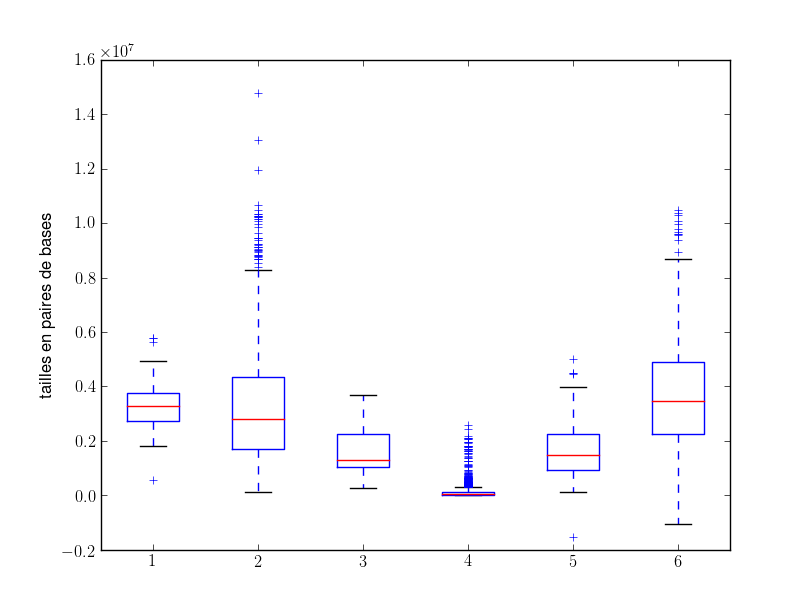
\includegraphics[width=0.9\textwidth]{./img/replicon_mustach.png}
		\caption{Tailles des génomes}\label{taille}
	\end{subfigure}
	\begin{subfigure}{0.6\textwidth}
		\centering
		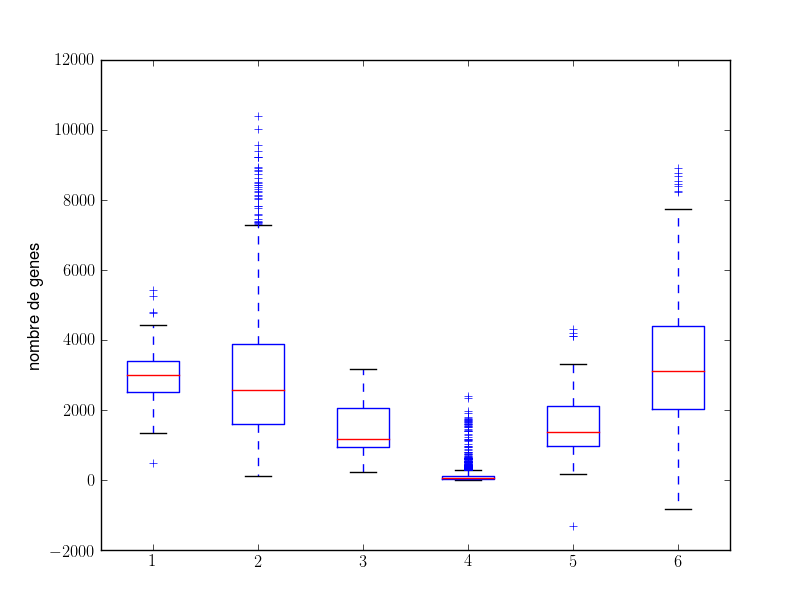
\includegraphics[width=0.9\textwidth]{./img/gene_mustach.png}
		\caption{Nombre de gènes}\label{nbgene}
	\end{subfigure}
	\caption[Distributions des tailles et nombres de gènes des réplicons]{Distributions des tailles (\ref{taille}) et nombres (\ref{nbgene}) de gènes des réplicons. \\
	Les boites délimitent les premiers et troisièmes quartiles (Q) des distributions, les limites des ``moustaches" inférieures et supérieures représentant respectivement Q1-1.5(Q3-Q1) et Q3+1.5(Q3-Q1). Les points en dehors des moustaches sont représentés par des croix. \textbf{1}: chromosomes des génomes multipartites. \textbf{2}: totalité des chromosomes. \textbf{3}: RECE. \textbf{4}: plasmides. \textbf{5}: différences des tailles (\ref{taille}) ou nombres de gènes (\ref{nbgene}) entre chromosome et RECE au sein d'un génome. \textbf{6}: différences des tailles (\ref{taille}) ou nombres de gènes (\ref{nbgene}) entre chromosome et plasmide au sein d'un génome.}\label{figsize}
\end{figure} 
	Ces facteurs ne sont pas suffisants pour caractériser les différents réplicons: Il existe des plasmides aussi grands que des RECE, et des RECE aussi grands que des chromosomes. Enfin, la répartition très inégale des génomes multipartites dans les différents groupes et genres bactériens (Figure \ref{specieplot}), pour des raisons évolutives ou historiques, crée un biais dans les données, biais dont il faudra tenir compte dans l'analyse.
\newpage
\usepgfplotslibrary{units}

\thispagestyle{empty}
\begin{figure}[H]
	\vspace{-2.5cm}	
      	\hspace{-2cm}
      	\begin{subfigure}{0.55\textwidth}
      		\begin{tikzpicture}
      		\tikzstyle{every node}=[font=\small]
\pie[cloud,scale font,sum=auto, color={purple!40,pink!60,magenta!80,red!60,cyan!60,blue!60,blue!40,green!10,lime!40,green!40,purple!1,black!20}]{1/,1/,2/,2/,2/,1/,2/,34/,47/,32/,7/,1/}
      		\end{tikzpicture}
      		\subcaption{Répartition des génomes multipartites à travers le domaine bactérien. Total:\textbf{133}}\label{fig1}
      \end{subfigure}
      \hspace{1cm}
      \begin{subfigure}{0.55\textwidth}
      	\begin{tikzpicture}
      	\tikzstyle{every node}=[font=\small]
      	\pie[cloud,scale font,sum=auto,color={purple!40,pink!60,magenta!80,red!60,cyan!60,blue!60,blue!40,green!10,lime!40,green!40,purple!1,black!20}]{1/,1/,1/,2/,2/,1/,2/,10/,4/,5/,1/,1/}
      	\end{tikzpicture}
       \subcaption{Répartition des genres bactériens ayant au moins un génome multipartite. Total:\textbf{31}}\label{diversite}
	 \end{subfigure}
      \\
      \\
      \vspace{1cm}
      \hspace{-4cm}
      \begin{subfigure}{1\textwidth}
      	\begin{tikzpicture}
      	\tikzstyle{every node}=[font=\small]
      	\pie[cloud,scale font,sum=auto,color={purple!40,pink!60,magenta!80,orange!40,red!60,cyan!60,blue!60,blue!40,green!10,lime!40,black!10,green!1,green!40,purple!1,brown!20,black!20}]{8/,345/,111/,110/,19/,82/,23/,745/,280/,168/,61/,109/,714/,82/,89/,104/}

      	\end{tikzpicture}
     {\advance\leftskip+3cm\subcaption{Répartition des génomes bactériens disponibles. Total:\textbf{3052}}}
    	\end{subfigure}
	\begin{subfigure}{1\textwidth}\label{fig2}
	\hspace{-3cm}
      	\begin{tikzpicture}
      	\tikzstyle{every node}=[font=\small]
      	\pie[cloud,scale font,sum=auto,text=legend,color={purple!40,pink!60,magenta!80,orange!40,red!60,cyan!60,blue!60,blue!40,green!10,lime!40,black!10,green!1,green!40,purple!1,brown!20,black!20}]{6/Acidobactéries,79/Actinobactéries,61/Bacteroidetes,6/Chlamydiae,11/Chloroflexi,34/Cyanobactéries,6/Deinococcus-Thermus,90/Firmicutes,72/Alphaprotéobactéries,49/Bêtaprotéobactéries,29/Deltaprotéobactéries,11/Epsilonprotéobactéries,104/Gammaprotéobactéries,9/Spirochètes,6/Ténéricutes,69/autres}

      	\end{tikzpicture}
      {\advance\leftskip+3cm\caption{Répartition des genres bactériens ayant au moins un génome disponible. Total:\textbf{638}}}
      \end{subfigure}
      \hspace*{-3cm}
      \begin{minipage}{1.37\textwidth}
      \medskip
      \caption[Répartition par lignée des génomes bactériens disponibles]{\scriptsize Répartition par lignée des génomes bactériens disponibles au 23/11/2013 dans la base de données RefSeq \citep{pruitt2007ncbi} classés selon la taxonomie bactérienne en vigueur (http://www.bacterio.net/).\\
       Seuls les génomes complets ont été pris en compte. Les génomes sont organisés selon le phylum de leur hôte sauf pour les Protéobactéries pour lesquels la classe a été utilisée. La catégorie ``Autres" regroupe les phylum faiblement représentés dans RefSeq: Aquificae, Chlorobi, Deferribacteres, Fibrobacteres, Fusobactéries, Gemmatimonadetes, Nitrospirae, Planctomycètes, Thermodesulfobactéries, Thermotogae, et Verrucomicrobia.}\label{specieplot}
       \end{minipage}       
\end{figure}


\section{Nature, origine et fonctionnement des RECE: une problématique ouverte}\label{justification}    
	
Jusqu'à maintenant, la problématique de ce que sont les RECE a été abordée principalement au cours d'études ponctuelles de génomes individuels et parfois, d'espèces bactériennes. Plusieurs tentatives de définition ont été faites \citep{Mackenzie2004}, la plus complète et récente étant celle de Harrison \citep{harrison2011bacterial}, sans pour autant clôturer le débat sur la nature chromosomique \textit{vs.} plasmidique des RECE. En effet, l'étude de Harrison ne s'attache qu'à la comparaison des RECE aux chromosome et plasmide(s) présents dans le même génome, et est majoritairement focalisée pour ce qui est de l'étude approfondie, sur une seule espèce
 (\textit{Burkholderia cenocepacia}) d'un seul genre (\textit{Burkholderia}) d'une seul famille (Burkholderiaceae). Ces résultats ne peuvent donc pas être directement généralisés à l'ensemble des RECE bactériens. Les travaux de Harrison \textit{et al.} \citep{Harrison2010, harrison2011bacterial} apportent néanmoins de précieuses observations, dont l'interprétation va au-delà de l'introduction de l'appellation de ``\textit{chromid}". En effet, la définition du \textit{chromid} revient à dire que les RECE fonctionnent comme des chromosomes mais ne peuvent être appelés chromosome parce qu'ils sont plasmidiques à l'origine. La question devient alors : \textbf{Qu'est-ce qu'un chromosome?} \\
	Les différents éléments présentés dans ces deux premiers chapitres mettent en évidence une continuité génomique entre plasmides, RECE et chromosomes, et révélent l'existence de mécanismes moléculaires et structures génomiques communs à ces différents types de réplicons. Cette similitude est d'autant plus affirmée qu'il devient difficile de discerner si certains réplicons sont des (méga)plasmides ou des chromosomes. Ainsi la définition même de RECE n'est pas appropriée, la distinction entre réplicons bactériens pouvant au final se résumer à deux éléments: leur essentialité pour l'organisme les hébergeant et leurs intégration et stabilisation dans le cycle cellulaire, leur rôle en étant une conséquence. Du point de vue de l'évolution du matériel génétique, les bactéries à génome multipartite représentent de fait une collection de données génomiques cruciale pour appréhender les nature et importance des forces évolutives mises en œuvre dans l'organisation du matériel génétique et la complexification et l'adaptation des génomes bactériens. Or, les études faites jusqu'à présent ne permettent pas de caractériser clairement et de manière générale ce que sont un plasmide, un chromosome ou un RECE parmi les réplicons bactériens. \\
       Les travaux de cette thèse portent sur la caractérisation des génomes multipartites par une \textbf{étude globale sans \textit{a priori} de l'ensemble des génomes bactériens et données disponibles dans les bases de données publiques} dont l'objectif est d'identifier des tendances générales des mécanismes génétiques impliqués dans l'apparition et la stabilisation des architectures génomiques multipartites. 























    